
\(f(x) = 60x \e^{-0{,}5x}\).

\subsection*{1.}

\( f \) est un produit de fonctions dérivables sur \( \mathbb{R} \), donc sur \([0 \,;\, 10]\) et sur cet intervalle :
\begin{align*}
f'(x) &= 60\e^{-0{,}5x} + 60x \times (-0{,}5)\e^{-0{,}5x} \\
&= \e^{-0{,}5x}(60 - 30x) \\
&= -30(x - 2)\e^{-0{,}5x}.
\end{align*}

\subsection*{2.}

On sait que, quel que soit le réel \( x \), \( \e^{-0{,}5x} > 0 \), donc le signe de \( f'(x) \) est celui de \( 2 - x \) :
\begin{align*}
&2 - x > 0 \\
\iff &2 > x \\
\iff &x < 2.
\end{align*}
Sur \([0 \,;\, 2]\), \( f'(x) > 0 \), sur \([2 \,;\, 10]\), \( f'(x) < 0 \) et \( f'(2) = 0 \).

\subsection*{3.}

D'après la question précédente \( f \) est croissante sur \([0 \,;\, 2]\) de \( f(0) = 0 \) à \( f(2) = 120\e^{-1} \approx 44{,}1 \), puis décroissante sur \([2 \,;\, 10]\) de \( f(2) = 120\e^{-1} \) à \( f(10) = 600\e^{-5} \approx 4{,}04 \). D'où le tableau :

\begin{center}
\begin{tikzpicture}
\tkzTabInit[lgt=3.5, espcl=4]{$x$ / 1, {Signe de $f'(x)$} / 1, {$f(x)$} / 2}{${0}$, ${2}$, ${10}$}
\tkzTabLine{,+,0,-,}
\tkzTabVar{-/{$0$},+/{$120\e^{-1}$},-/{$600\e^{-5}$}}{/}
\end{tikzpicture}
\end{center}

\subsection*{4.}
On a vu que \( f'(2) = 0 \) : le coefficient directeur de la tangente à la courbe représentative de la fonction \( f \) est parallèle à l'axe des abscisses (horizontale).

\subsection*{5.}

On sait qu'une équation réduite de la tangente à la courbe représentative de la fonction \( f \) au point d'abscisse 0 est :
\[
y - f(0) = f'(0)(x - 1).
\]
Avec :
\[
f(0) = 0 \quad \text{et} \quad f'(0) = -30(0 - 2)\e^{-0{,}5 \times 0} = 60 \e^0 = 60 \times 1 = 60,
\]
l'équation devient \(y = 60x\).

